%
% fig-parallel.tex
%
% (c) 2025 Prof Dr Andreas Müller
%
\begin{figure}
\centering
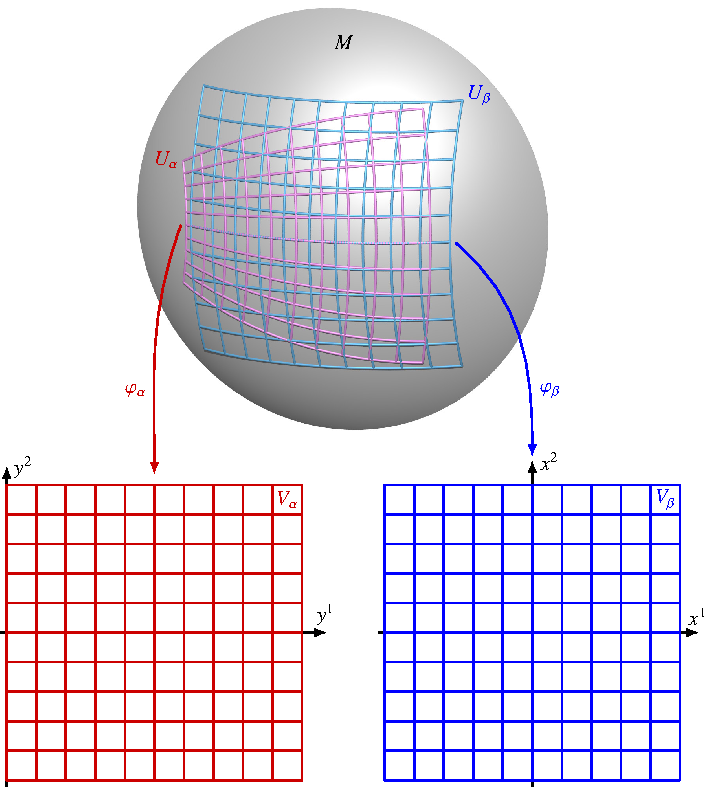
\includegraphics{chapters/020-koordinaten/images/parallel.pdf}
\caption{Je nach Koordinatensystem (Karte) hat ein entlang einer
Koordinatenlinie in der Karte parallel transportierter Vektor
eine ganz andere Richtung.
Dies illustriert, dass es ohne das zusätzliche Konzept eines
Zusammenhangs nicht möglich ist, benachbarte Vektoren zu vergleichen
oder Vektoren abzuleiten.
\label{buch:koordinaten:diffop:fig:transport}}
\end{figure}
